	%!TEX root = ../../Main.tex
\graphicspath{{Chapters/Krav/}}
%-------------------------------------------------------------------------------


\section{Krav}
I dette afsnit beskrives kravene til CSS og hvilken funktionalitet systemet skal have. Der er stillet nogle enkelte krav fra kursets side, hvor nogle af disse krav skal indgå i projektet:

\begin{itemize}
	\item Use In Circuit debug tools
	
	\item Implement Drivers, dealing with time critical parameters.
	
	\item Implement Boot Loaders for updating microcontroller firmware
	
	\item Use USB to interface a microcontroller
	
	\item Use operating systems for microcontrollers
	
	\item Use microcontroller knowledge in a final mini project
	
\end{itemize}

Flere af disse krav er implementeret i CSS. Der er brugt tidskritiske drivers til color sensoren, display modulet og til implementeringen af I2C mellem de to microcontrollers. 

\begin{figure}[H]
	\centering
	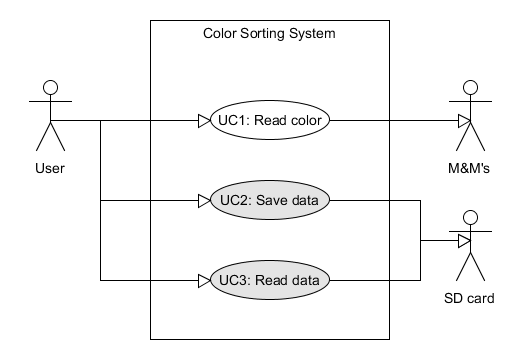
\includegraphics[width = 400pt]{Img/Usecase_diagram.png}
	\caption{Usecase diagram for CSS}
	\label{fig:UsecaseDiagram}
\end{figure}

På \autoref{fig:UsecaseDiagram} ses usecase diagrammet som beskriver sammenhængen mellem aktørerne og de forskellige funktionaliteter der findes for systemet. Uscase 2 og 3 er grå, hvilket betyder at de ikke er implementeret i prototypen. 

\subsection{UC1 - Read Color}
Denne usecase danner ramme for, hvordan CSS måler en farve. Brugeren placerer emne der ønsket aflæst. Brugeren trykker på aflæs-knappen og den aflæste farve kan nu ses talt op på TFT display modulet.

\subsection{UC2 - Save Data}
Denne usecase danner ramme for, at gemme data på SD kort. Brugeren trykker på "Save Data" knappen på skærmen. Data bliver derefter gemt på SD kort.

\subsection{UC3 - Read Data}
Denne usecase danner ramme for, at hente data fra SD kortet. Brugeren trykker på "Load Data" knappen på skærmen. Gemt data bliver hentet fra SD kortet og vist på TFT skærmen.

\subsection{Afgrænsning}
Det skal siges, at usecase 2 og 3 ikke er implementeret i denne protorype. Der er gjort forsøg på at få dem implementeret, men grundet tidspres blev de nedprioriteret. Derudover var det også tænkt fra start, at der ikke skulle være behov for brugerinput for at kunne aflæse farve, men på grund af tidsmangel fik gruppen ikke implementeret et system der kunne fodre CSS med emner. Dette gøres istedet for manuelt og vil i fremtiden skulle noget automatisering af CSS implementeres.

